% LaTeX source for ``การเรียนรู้ของเครื่องสำหรับเคมีควอนตัม (Machine Learning for Quantum Chemistry)''
% Copyright (c) 2022 รังสิมันต์ เกษแก้ว (Rangsiman Ketkaew).

% License: Creative Commons Attribution-NonCommercial-NoDerivatives 4.0 International (CC BY-NC-ND 4.0)
% https://creativecommons.org/licenses/by-nc-nd/4.0/

\chapter{โมเดลการเรียนรู้ของเครื่องสำหรับเคมีควอนตัม}
\label{ch:chem_ml}

%--------------------------
\section{ANI-1}
\label{sec:ani1}
\idxen{Model for Quantum Chemistry!ANI-1}
%--------------------------

ANI เป็นชื่อย่อสั้น ๆ ของโมเดล ANAKIN-ME ซึ่งย่อมาจาก Accurate NeurAl networK engINe for Molecular Energies อีกทีหนึ่ง 
ซึ่งผู้เขียนคิดว่าผู้พัฒนาน่าจะตั้งชื่อเพื่อให้มีตัวย่อตรงกับ Artificial Narrow Intelligence (ANI) หรือการเรียนรู้แบบแคบ%
\footnote{Artificial Narrow Intelligence เป็นเทคนิคปัญญาประดิษฐ์แบบหนึ่งซึ่งจะถูกออกแบบให้มีความสามารถและเชี่ยวชาญเฉพาะด้าน}
โดยโมเดลตัวนี้ถูกพัฒนาด้วย Neural Network สำหรับการทำนายค่าพลังงานศักย์ของโมเลกุลโดยที่มีความแม่นยำในระดับเดียวกับการคำนวณด้วยวิธี 
DFT\autocite{smith2017}

%--------------------------
\section{Deep Tensor Neural Network}
\label{sec:dtnn}
\idxen{Model for Quantum Chemistry!Deep Tensor Neural Network}
%--------------------------

\autocite{schutt2017a}

%--------------------------
\section{SchNet และ SchNOrb}
\label{sec:schnet_schnorb}
%--------------------------

%--------------------------
\subsection{SchNet}
\label{ssec:schnet}
\idxen{Model for Quantum Chemistry!SchNet}
%--------------------------

SchNet เป็นโมเดลที่ใช้ Continuous Convolutions ซึ่งได้แรงบันดาลใจมาจาก Convolutional Neural Network (CNN) สำหรับการ%
อธิบายอัตรกิริยาระหว่างอะตอม\autocite{schutt2017,schutt2018}

%--------------------------
\subsection{SchNOrb}
\label{ssec:schnorb}
\idxen{Model for Quantum Chemistry!SchNOrb}
%--------------------------

SchNOrb ย่อมาจาก \enquote{SchNet for Orbitals}\autocite{schutt2019a}

%--------------------------
\section{SchNarc}
\label{sec:schnarc}
\idxen{Model for Quantum Chemistry!SchNarc}
%--------------------------

SchNarc เป็นโมเดล ML สำหรับการศึกษาพลศาสตร์โมเลกุลที่สภาวะกระตุ้น (Excited State Dynamics)\autocite{westermayr2020} 
โดยเป็นการนำเอาโมเดล SchNet\autocite{schutt2017,schutt2018} มารวมกับอัลกอริทึม SCHARC\autocite{richter2011,mai2018} 
ซึ่งเป็นวิธี Semiclassical Surface Hopping

%--------------------------
\section{Symmetric Gradient Domain Machine Learning}
\label{sec:sgdml}
\idxen{Model for Quantum Chemistry!Symmetric Gradient Domain Machine Learning}
%--------------------------

\autocite{chmiela2017}

\autocite{chmiela2018}

\autocite{sauceda2020}

\autocite{chmiela2020}

\autocite{chmiela2022}

%--------------------------
\section{\texorpdfstring{$\Delta$}-ML}
\label{sec:delta_ML}
\idxen{Model for Quantum Chemistry!$\Delta$ML}
%--------------------------

งานวิจัยที่ใช้ผลต่างระหว่างผลการคำนวณด้วยวิธีที่มีความแม่นยำต่ำและวิธีที่มีความแม่นยำสูงมาเป็นค่าสำหรับการเพิ่มความถูกต้อง (Correction) 
เพื่อช่วยให้การคำนวณหรือทำนายคุณสมบัติของโมเลกุลมีค่าแม่นยำมากยิ่งขึ้นนั้นนั้นมีมานานแล้ว\autocite{hu2003,wu2007,balabin2009} 
โดยไอเดียนี้ก็ได้ถูกนำมาใช้ในงานวิจัย ML เช่นเดียวกัน ซึ่งเทคนิคนี้เรียกว่า Delta-ML ($\Delta$ML) 

$\Delta$ML เป็นเทคนิคที่ใช้ค่าความแตกต่างระหว่างค่าอ้างอิง (Reference หรือจะเรียก Label ก็ได้) จากวิธีการคำนวณที่มีความแม่นยำแตกต่าง%
กันมาใช้ในการเทรนโมเดล (จึงเป็นที่มาว่าทำไมถึงเรียกว่า Detla) โดยความแตกต่างนั้นอาจจะแตกต่างกันในบริบทของระดับ (Level) ของวิธีการ 
เช่น ใช้วิธี DFT เหมือนกันแต่ว่าใช้ Basis Set ที่ต่างกัน หรือจะใช้วิธีที่แตกต่างกันก็ได้ เช่น ใช้วิธี DFT และวิธี Coupled Cluster (ใช้ Basis 
Set เดียวกัน) ซึ่งการทำ Correction แบบนี้ด้วย $\Delta$ML สามารถช่วยให้โมเดลเพิ่มความสามารถในการถ่ายโอนการเรียนรู้ในการทำนาย 
(Transferability) ไปยังชุดข้อมูลทดสอบที่ต้องการทำนายได้อย่างถูกต้องและแม่นยำมากขึ้น โดยจะมีความถูกต้องเทียบเคียงกับการใช้วิธีแบบ%
ดั้งเดิมที่มีความแม่นยำสูง เช่น Post-HF ตามที่ได้อธิบายไป 

ตัวอย่างของการใช้ $\Delta$ML คือการใช้ค่าความแตกต่างของพลังงานที่ได้จากการคำนวณด้วยวิธี DFT และ CCSD(T) ซึ่งวิธี CCSD(T) นี้เปรียบ%
เสมือนเป็นวิธีมาตรฐานที่ให้ผลที่มีความแม่นยำสูงมาก (วิธี CCSD(T) ได้ฉายาว่าเป็น Gold Standard Method) โดยมี Correction ดังนี้

\begin{equation}\label{eq:diff_dft_cc}
    y_{\text{DFT}} - y_{\text{CCSD(T)}}
\end{equation}

ซึ่ง Raghunathan Ramakrishnan และทีมวิจัยได้นำเทอมในสมการที่ \ref{eq:diff_dft_cc} มาใช้ในการฝึกสอนโมเดล ML ซึ่งได้รับความ%
สนใจในช่วงเวลาต่อมา\autocite{ramakrishnan2015a} นอกจากนี้ยังมีงานวิจัยที่พัฒนา Graph Neural Network (GNN) และประยุกต์ใช้เข้า%
กับเทคนิค $\Delta$-learning สำหรับการประมาณค่าพลังงานส่วนต่างของเทอม Triple Excitation (Electronic Correction) 
เพื่อเพิ่มความแม่นยำในการทำนายค่าพลังงานให้มีความแม่นยำในระดับเดียวกันหรือใกล้เคียงกับวิธี CCSD(T)\autocite{ruth2022}

จริง ๆ แล้ว $\Delta$ML ก็เป็นเทคนิคอันหนึ่งที่มีแนวคิดมาจากความพยายามที่ต้องการจะทำให้โมเดลสามารถเรียนรู้ได้จากค่าความผิดพลาด (Error) 
โดยเริ่มมีการเอามาใช้กันมากขึ้นในช่วงปีที่ผ่านมา (ในช่วงแรกถูกใช้เยอะแค่ในเฉพาะกลุ่มวิจัยในโซนยุโรป สำหรับการเอามาทำนายพลังงานและ%
เกรเดียนต์ของพลังงาน (Energy Gradient) ซึ่งก็สอดคล้องกับแรงของแต่ละอะตอมในโมเลกุล รวมไปถึง Stationary Points บนพื้นผิว%
พลังงานศักย์ โครงสร้างที่สภาวะทรานซิชั่น (Transition State Structure) และที่สภาวะสมดุลด้วย

%--------------------------
\section{Graph Neural Network}
\label{sec:gnn}
\idxth{โครงข่ายประสาทแบบกราฟ}
\idxen{Graph Neural Network}
%--------------------------

โครงข่ายประสาทแบบกราฟ (Graph Neural Network หรือ GNN) เป็นโครงข่ายประสามแบบหนึ่งซึ่งจะมองความสัมพันธ์ภายในโครงสร้างข้อมูลให้%
อยู่ในรูปแบบของกราฟแบบ 2 มิติ โดยไอเดียนี้ได้ถูกเสนอตั้งแต่ปี ค.ศ. 2008\autocite{scarselli2009,zhou2020} โมเดล GNN นั้นได้รับ%
ความนิยมสูงมากในช่วงไม่กี่ปีที่ผ่านมานี้ (นับตั้งแต่ปี ค.ศ. 2018) โดย George Karypis นักวิทยาศาสตร์อาวุโสของบริษัท AWS ได้กล่าวไว้ใน%
การสัมมนาครั้งหนึ่งว่า 

\blockquote{GNNs are one of the hottest areas of deep learning research, and we see an increasing number of 
applications take advantage of GNNs to improve their performance}

\noindent ซึ่งถ้าหากเราไปดูจำนวนบทความงานวิจัยที่ตีพิมพ์ในช่วงที่ผ่านมาจะพบว่า GNN ได้ถูกนำมาใช้เยอะมาก นอกจากนี้ยังได้มีบริษัทชั้นนำทาง%
ด้านเทคโนโลยีต่าง ๆ ที่ให้ความสำคัญและความสนใจกับการพัฒนาโมเดล GNN เป็นอย่างมาก โดยหนึ่งในตัวอย่างที่ชัดเจนก็คือทีม AWS AI ได้พัฒนา%
ไลบรารี่สำหรับ GNN โดยเฉพาะ ชื่อว่า Deep Graph Library (DGL) โดยผู้อ่านสามารถดูรายละเอียดได้ที่ \url{https://www.dgl.ai}

สำหรับโมเดล GNN ที่ผู้อ่านจะได้ศึกษาในหัวข้อนี้ก็คือ Message Passing Neural Network ซึ่งเป็นหนึ่งในโมเดล GNN ที่มีประสิทธิภาพในการ%
ทำนายคุณสมบัติเชิงอิเล็กทรอนิกส์ของโมเลกุลสูงมาก

\begin{figure}[htbp]
    \centering
    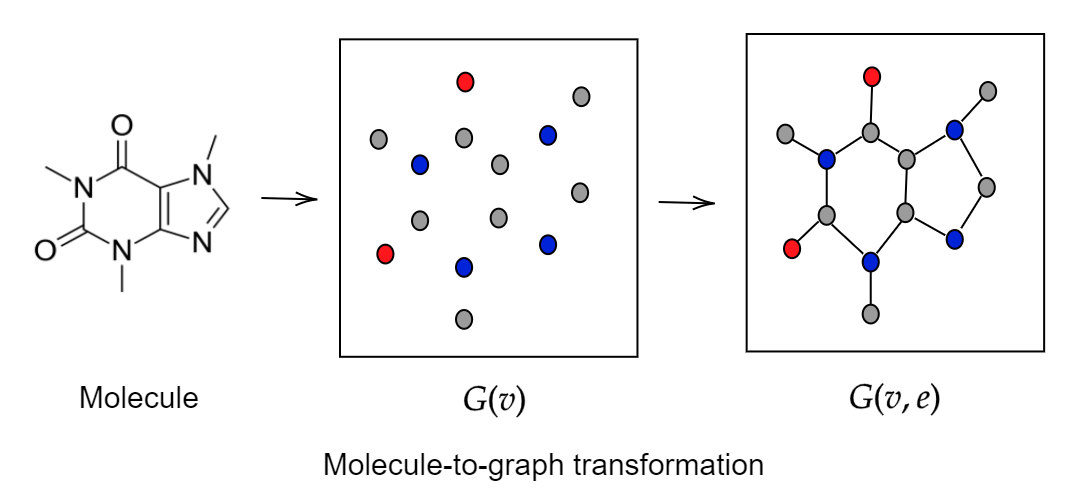
\includegraphics[width=\linewidth]{fig/mol-2-graph.png}
    \caption{การแทนโมเลกุลด้วยกราฟ}
    \label{fig:mol_2_graph}
\end{figure}

ภาพ \ref{fig:mol_2_graph} แสดงกราฟฟิคของการเปรียบเทียบโมเลกุลและกราฟ ซึ่งจะเห็นได้ว่าการแปลงจากโมเลกุลไปเป็นกราฟนั้นสามารถ%
ทำได้ตรงไปตรงมาเพราะว่าเราสามารถแทนอะตอมด้วยโหนด (Node) หรือจุดยอดของกราฟ (Vertex) และแทนพันธะด้วยขอบ (Edge)

%--------------------------
\subsection{MatErials Graph Network}
\label{ssec:megnet}
\idxth{โครงข่ายประสาทแบบกราฟ!โครงข่ายกราฟสำหรับวัสดุ}
\idxen{Graph Neural Network!MatErials Graph Network}
%--------------------------

หนึ่งในโมเดล GNN ที่ได้มีประสิทธิภาพในการทำนายคุณสมบัติของโมเลกุลขนาดเล็กและโมเลกุลขนาดใหญ่คือโมเดล MatErials Graph Network 
(MEGNet)\autocite{chen2019}

ผู้อ่านสามารถดูรายละเอียดของซอร์สโค้ดของโปรแกรม MEGNet ได้ที่ \url{https://github.com/materialsvirtuallab/megnet}

%--------------------------
\section{Message Passing Neural Network}
\label{sec:mpnn}
\idxth{โครงข่ายประสาทแบบการส่งข้อความ}
\idxen{Message Passing Neural Network}
%--------------------------

โครงข่ายประสาทแบบการส่งข้อความ (Message Passing Neural Network หรือ MPNN) เป็น GNN ประเภทหนึ่งซึ่งถูกนำเสนอครั้งแรกเมื่อปี 
ค.ศ. 2017\autocite{gilmer2017} โดยที่ MPNN แบบฉบับดั้งเดิมนั้นจะเป็นการใช้กราฟแบบที่ไม่มีการนำทิศทางหรือ Undirected Graph
ซึ่ง MPNN นั้นประกอบไปด้วยเฟสหลัก 2 เฟส ดังนี้ 

\begin{itemize}
    \item Message Passing Phase เฟสการส่งผ่านข้อมูลซึ่งอยู่ในรูปของข้อความ เป็นเฟสที่จะทำการขยับหรือแผ่กระจายข้อมูลไปทั่วทั้งกราฟ%
    เพื่อจำลองการเกิด Neural Network และการส่งต่อข้อมูลจากโหนดหนึ่งไปยังอีกโหนดหนึ่ง
    
    \item Readout Phase เฟสการเรียกใช้ข้อมูล เป็นเฟสที่ Neural Representation ของกราฟจะถูกใช้ในการทำนายค่าของเอาต์พุต เช่น
    คุณสมบัติของแต่ละโหนด ซึ่งเปรียบเสมือนการทำนายคุณสมบัติของแต่อะตอมแต่ละตัวในโมเลกุลนั่นเอง
\end{itemize}

%--------------------------
\subsection{สถาปัตยกรรม}
\label{ssec:mpnn_architect}
\idxth{โครงข่ายประสาทแบบการส่งข้อความ!สถาปัตยกรรม}
\idxen{Message Passing Neural Network!Architecture}
%--------------------------

\begin{figure}[htbp]
    \centering
    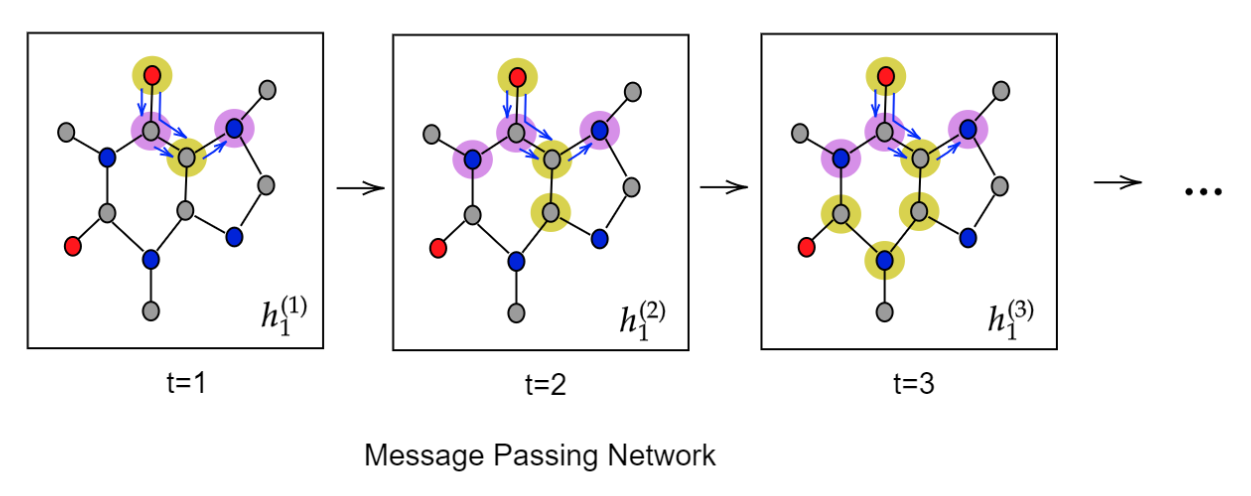
\includegraphics[width=\linewidth]{fig/mp-network.png}
    \caption{โครงข่ายของการส่งข้อความ}
    \label{fig:mp_network}
\end{figure}

เรามาดูรายละเอียดของสถาปัตยกรรมของ MPNN กันครับ เริ่มที่เฟสแรกซึ่งเป็นการดำเนินการแผ่กระจายข้อมูลทั่วทั้งกราฟ โดยจำนวนก้าวที่ใช้ในการทำ 
Propagation นั้นจะเขียนแทนด้วย $T$ ซึ่งจริง ๆ แล้วก็คือจำนวนรอบของการฝึกสอนโมเดล (Iteration) นั่นเอง นอกจากนี้เรายังกำหนดตัวแปร%
แทนพารามิเตอร์อื่น ๆ อีก ดังนี้

\begin{description}[font=$\bullet$,labelindent=2em,labelwidth=2cm,labelsep=0em]
    \item[\ $h$] สถานะซ่อน
    
    \item[\ $m^{t}_{v}$] ข้อความของโหนด $v$ ณ สเต็ปที่ $t$
    
    \item[\ $M$] ฟังก์ชันที่ใช้ในการอัพเดทข้อความ
    
    \item[\ $U_{t}$] ฟังก์ชันที่ใช้ในการอัพเดทโหนด ณ สเต็ปที่ $t$    
\end{description}

\noindent ซึ่งฟังก์ชันที่ใช้ในการอัพเดทข้อความของแต่ละเสต็ปที่เกิดขึ้นในการกระบวน Propagation นั้นมีหน้าตาดังนี้

\begin{equation}\label{eq:msg_func}
    m^{t+1}_{v} = \sum_{w \in N(v)} M_{t} (h^{t}_{v}, h^{t}+{w}, e_{vw})
\end{equation}

ถ้าหากสังเกตสมการที่ \ref{eq:msg_func} ดี ๆ จะพบว่าฟังก์ชัน $m$ จะมีการดำเนินการนำข้อมูลของสถานะซ่อน (Hidden States) ของ%
โหนด $w$ เข้าไปกระทำกับโหนด $v$ และยังมีการนำข้อมูลของขอบระหว่างโหนด $e_{vw}$ เข้ามารวมไว้ในฟังก์ชันด้วย นอกจากนี้สมการทาง%
คณิตศาสตร์ของ Hidden State สามารถเขียนให้อยู่ในรูปของฟังก์ชันที่ใช้อัพเดทสถานะของแต่ละโหนดได้ดังนี้ 

\begin{equation}\label{hidden_func}
    h^{t+1}_{v} = U_{t}(h^{t}_{v}, m^{t+1}_{v})
\end{equation}

\noindent โดยที่ $N(v)$ คือเซตของโหนดข้างเคียงของโหนด $v$ ในกราฟ $G$ และ $h^{0}_{v}$ คือฟังก์ชันเริ่มต้น (ฟังก์ชันอะไรก็ได้) 
สำหรับการกำหนดค่าเริ่มต้นของข้อมูลของโหนดนั้น ๆ (กำหนด Feature) $x_{v}$

\begin{center}
\fbox{%
\begin{minipage}[c][3.5cm]{0.8\linewidth}
    \null\,\, $\phi_{1 \rightarrow 3} = f(v_{1} \rightarrow v_{3})$ \\
    \null\,\, $\psi_{2 \rightarrow 3} = f(v_{2} \rightarrow v_{3})$ \\
    \null \hspace{2em} Summarize messages: $\Omega = \phi_{1 \rightarrow 3} \,\, \& \,\, 
    \psi_{2 \rightarrow 3}$ \\
    \\
    \null\,\, $h^{t+1}_{v} = \text{Update}(h^{t}_{v}, \Omega )$
\end{minipage}}
\end{center}

เมื่อเรามีสถานะซ่อนของแต่ละโหนด ณ เวลาที่แตกต่างกันแล้ว ($h^{t}_{v}$) ลำดับถัดมาคือเราต้องการดำเนินการถดถอย (Regress) สถานะซ่อน%
ทั้งหมดนี้เพื่อคำนวนความสัมพันธ์ไปยังค่าเอาต์พุตนั่นเอง ซึ่งกระบวนการหรือสิ่งที่เราจะนำมาใช้ในการทำดังกล่าวคือต้องใช้ฟังก์ชัน Readout $R$ นั่นเอง
หรือพูดง่าย ๆ คือเป็นฟังก์ชันที่ใช้ในการถอดข้อความออกมาเป็นเอาต์พุต เรียกว่าการทำนายสถานะซ่อน โดยมีสมการดังต่อไปนี้

\begin{equation}
    \hat{y} = R({h^{T}_{v} | v \in G})
\end{equation}

\noindent ฟังก์ชัน Readout ที่เราจะนำมาใช้นั้นจะเป็นฟังก์ชันอะไรก็ได้ ขอแค่สามารถรวบรวม (Compose) ข้อความทั้งหมดที่อยู่ในรูปของสถานะ%
ซ่อนเข้าไว้ด้วยกันและทำการผสาน (Merge) ข้อความเหล่านั้นให้เป็น $\hat{y}$ ซึ่งวิธีที่ง่ายที่สุดที่สามารถนำมาใช้ในการรวมรวมสถานะต่าง ๆ 
เข้าไว้ด้วยกันก็คือการใช้ฟังก์ชันการรวมแบบเชิงเส้น (Linear Combination)

\begin{equation}
    h = \sum_{v \in G} h^{T}_{v}
\end{equation}

\begin{equation}\label{eq:ff_mpnn}
    \hat{y} = f(h)
\end{equation}

สุดท้ายแล้วจุดประสงค์ของการฝึกสอนโมเดล MPNN ก็คือฟังก์ชันที่รับสถานะของแต่ละโหนดเข้ามาที่ผ่านการแผ่กระจายมาจากโหนดอื่น ๆ โดยผ่าน%
ขอบระหว่างโหนด แล้วทำการรวมข้อมูลและแปลงให้เป็นคำตอบที่ต้องการทำนาย สมการที่ \ref{eq:ff_mpnn} ก็คือการฝึกสอนโมเดล 
Feed-Forward Neural Network โดยใช้ฟังก์ชันแบบไม่เชิงเส้น (Nonlinear) $f$

\begin{figure}[htbp]
    \centering
    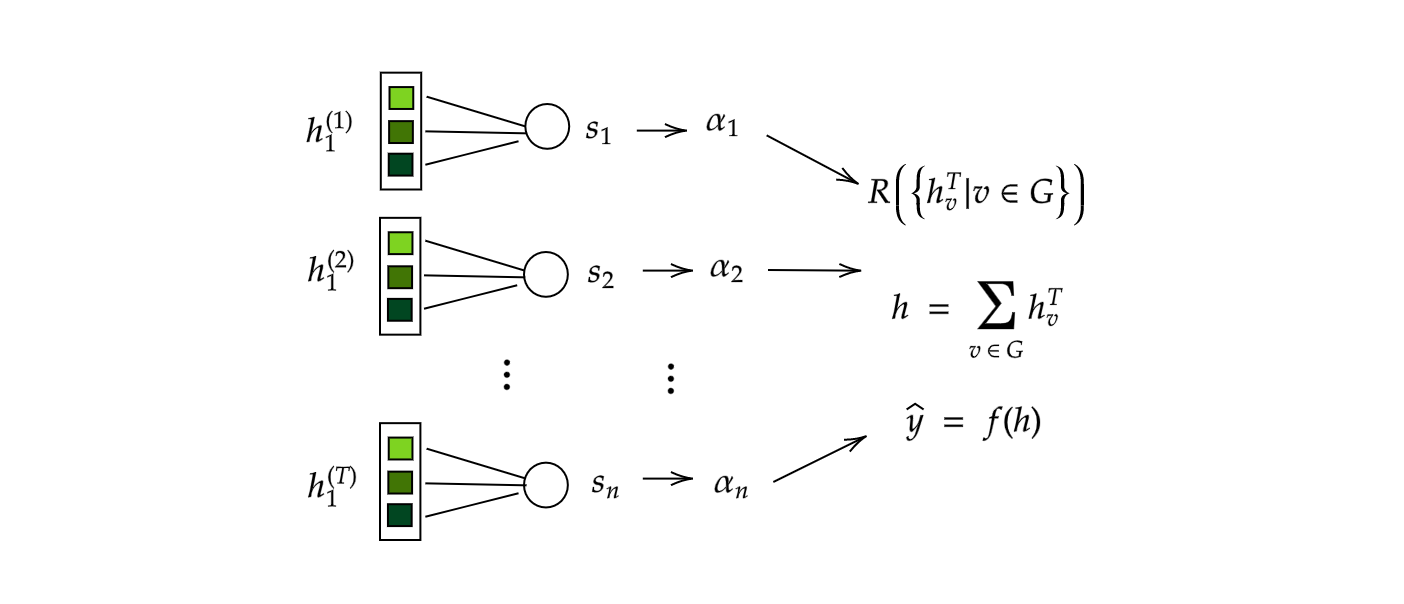
\includegraphics[width=0.9\linewidth]{fig/mp-operation.png}
    \caption{การดำเนินการของการทำการถดถอย (Regression) และการเรียกหรือดึงข้อมูลโดยใช้ Readout}
    \label{fig:mp_operation}
\end{figure}

สำหรับ Representation ของโมเลกุลที่เราสามารถเลือกใช้เพื่อนำฝึกสอนโมเดล MPNN นั้นจะแบ่งออกได้ง่าย ๆ ตามลักษณะองค์ประกอบของกราฟ 
นั่นคือ \textit{โหนด} ซึ่งเรามองเห็นอะตอม และ \textit{ขอบ} ซึ่งเรามองเห็นพันธะระหว่างอะตอม ดังนี้

\noindent \textbf{อะตอม}

\begin{itemize}[topsep=0pt]
    \item ชนิดของอะตอม (Atom Type)
    
    \item ขั้นของอะตอม (Atom Degree)
    
    \item จำนวนเวเลนซ์อิเล็กตรอน (Valence Electrons)
    
    \item ประจุฟอร์มอล (Formal Charge)
    
    \item จำนวนอิเล็กตรอนอิสระ (Radical Electrons)
    
    \item ไฮบริไดเซชั่น (Hybridization) เช่น SP, SP$^2$, SP$^3$, SP$^3$D, SP$^3$D$^2$
    
    \item ความเป็นอะโรมาติก (Aromaticity)
    
    \item จำนวนไฮโดรเจนอะตอม (Hydrogen Atoms)
    
    \item จำนวนหมู่ฟังก์ชัน (Functional Groups)
\end{itemize}

\medskip

\noindent \textbf{พันธะเคมี}

\begin{itemize}[topsep=0pt]
    \item ความยาวพันธะ
    
    \item ชนิดของพันธะ
    \begin{itemize}[topsep=0pt]
        \item พันธะเดี่ยว (Single Bond)
        
        \item พันธะคู่ (Double Bond)
        
        \item พันธะสาม (Triple Bond)
        
        \item พันธะแบบอื่น ๆ เช่น พันธะของอะโรมาติก
    \end{itemize}
\end{itemize}

นอกจากนี้ ในปี ค.ศ. 2021 นักวิจัยจากมหาวิทยาลัยเทคนิคแห่งเบอร์ลิน (Technical University of Berlin) ประเทศเยอรมัน นำโดย 
Kristof T. Sch\"{u}tt ได้ตีพิมพ์งานวิจัยซึ่งได้นำเสนออัลกอริทึมที่ชื่อว่า Equivariant Message Passing และสถาปัตยกรรมแบบใหม่ชื่อว่า 
Polarizable Atom Interaction Neural Network (PaiNN)\autocite{schutt2021} โดยวัตถุประสงค์ก็คือเป็นการแก้ปัญหาที่เกี่ยวข้อง%
ความสมมาตรของโมเลกุลของอัลกอริทึม MPNN แบบปกติ

ผู้อ่านสามารถศึกษาโค้ดสำหรับการคำนวณ Feature ของโหนดและขอบและโค้ดการสร้างโมเดล MPNN โดยใช้ TensorFlow และ Keras ได้ที่
\url{https://github.com/rangsimanketkaew/mpnn}

%--------------------------
\subsection{งานวิจัยที่เกี่ยวข้องกับ Message Passing Neural Network}
\label{ssec:mpnn_papers}
%--------------------------

เนื่องจากในปัจจุบันนั้นได้มีงานวิจัยที่ได้มีการนำ GNN มาใช้พัฒนาและต่อยอดเป็นจำนวนมาก ผู้เขียนจะขอยกตัวอย่างงานวิจัยที่ผู้เขียนคิดว่าน่าสนใจ 
โดยหนึ่งในนั้นก็คือ \enquote{การพัฒนา Descriptor โดยใช้กราฟ สำหรับการทำนายคุณสมบัติของพอลิเมอร์}\autocite{aldeghi2022} 
ซึ่งในงานวิจัยนี้ผู้วิจัยได้เลือกใช้ Weighted Directed Message Passing Neural Network (wD-MPNN) ซึ่งเป็น GNN ประเภทหนึ่ง และ 
Descriptor ที่ได้พัฒนาขึ้นมานั้นจริง ๆ แล้วก็คือเป็นการนำ Molecular Graph ที่มีอยู่แล้วนำมาปรับเพิ่มความสามารถในการบ่งบอกหรือเป็นตัวแทน 
(Represent) ความเป็นพอลิเมอร์ให้ดียิ่งขึ้น%
\footnote{บทความงานวิจัย A Graph Representation of Molecular Ensembles For Polymer Property Prediction โดย 
Matteo Aldeghi และ Connor W. Coley} 
โดยในงานวิจัยนี้ผู้วิจัยได้เพิ่มพจน์ \enquote{Stochastic Edges} เข้าไปในโมเดล wD-MPNN เพื่อให้อธิบาย Repeating Unit ของพอลิเมอร์%
ดียิ่งขึ้น (พอลิเมอร์เกิดจากมอนอเมอร์ซ้ำ ๆ กัน หลาย ๆ ตัวมาต่อกัน) สิ่งที่น่าสนใจคือปกติแล้ว GNN จะมีประสิทธิภาพในการทำนายคุณสมบัติของ%
โมเลกุลในกรณีที่เป็น Isolated Molecule (โมเลกุลที่อยู่ตัวเดียวโดด ๆ) ได้ดีมาก ๆ แต่กรณีของพอลิเมอร์ที่เป็นโครงข่ายที่มีขนาดใหญ่มากนั้น 
ความท้าทายคือเราจะจัดการกับอันตรกิริยาหรือปฏิสัมพันธ์ระหว่าง Repeating Unit อย่างไร ? สรุปโจทย์ง่าย ๆ ก็คือเราจะสอนให้โมเดล GNN 
รู้ได้อย่างไรว่ามีโมเลกุลอื่น ๆ อีกหลายโมเลกุลที่มาต่อหรือสร้างพันธะกับโมเลกุลเริ่มต้นออกไปทั้งทางซ้ายและขวาเพื่อให้มีความเป็นพอลิเมอร์มากที่สุด 

สิ่งที่งานวิจัยชิ้นนี้ทำนายก็คือค่า Electron Affinity (EA) กับ Ionization Potential (IP) ของโมเลกุลโคพอลิเมอร์ (Copolymer) 
จำนวนทั้งหมด 42,966 พอลิเมอร์ ซึ่งค่าอ้างอิงของ EA กับ IP นั้นก็ถูกคำนวณโดยใช้ทฤษฎี DFT ซึ่งโดยตัวส่วนตัวแล้วผู้เขียนคิดว่างานวิจัยนี้ยัง%
สามารถต่อยอดได้อีกเยอะเพราะว่าจริง ๆ แล้วยังมีคุณสมบัติอื่น ๆ ของพอลิเมอร์ที่ท้าทายกว่า EA กับ IA มาก เช่น คุณสมบัติเชิงกล (Mechanical 
Properties) ซึ่งถ้าหากเราสามารถพัฒนาโมเดล ML ที่ทำนายคุณสมบัติเหล่านี้ได้อย่างแม่นยำ ก็น่าจะเป็นประโยชน์ต่อฝั่งนักทดลองพอลิเมอร์แน่นอน
ถ้าหากผู้อ่านสนใจรายละเอียดเพิ่มเติมก็ไปลองอ่านงานวิจัยฉบับเต็มได้ บทความฉบับนี้อ่านง่าย ไม่ลงทฤษฎีเยอะมาก

%--------------------------
\section{Generative Adversarial Network}
\label{sec:gan}
\idxen{Generative Adversarial Network}
%--------------------------

Generative Adversarial Network (GAN) เป็น Generative Model แบบหนึ่งซึ่งเป็น Unsupervised ML โดยผู้ที่นำเสนอไอเดียของ GAN 
ก็คือ Ian Goodfellow โดยได้เผยแพร่บทความวิชาการในปี ค.ศ. 2014\autocite{goodfellow2014b} สำหรับผู้อ่านที่สนใจรายละเอียดของ 
GAN และแอพพลิเคชั่น ผู้เขียนแนะนำให้อ่านบทความ \enquote{18 Impressive Applications of Generative Adversarial Networks 
(GANs)} บทเว็บไซต์ Machine Learning Mastery%
\footnote{\url{https://machinelearningmastery.com/impressive-applications-of-generative-adversarial-networks}}

\noindent โดยรูปแบบโครงสร้างของ GAN ประกอบไปด้วยองค์ประกอบหลัก 2 ส่วน ดังนี้

\begin{enumerate}
    \item Generator คือโมเดลที่ถูกฝึกสอนให้มีความสามารถในการการสร้างตัวอย่างขึ้นมาใหม่โดนการสุ่มความแปรปรวนจากข้อมูลเริ่มต้น
    \idxen{Generative Adversarial Network!Generator}
    \item Discriminator คือโมเดลที่ถูกฝึกฝนให้มีความสามารถในการการจำแนกตัวอย่างจริงหรือตัวอย่างปลอมออกจากกัน
    \idxen{Generative Adversarial Network!Discriminator}
\end{enumerate}

\begin{figure}[htbp]
    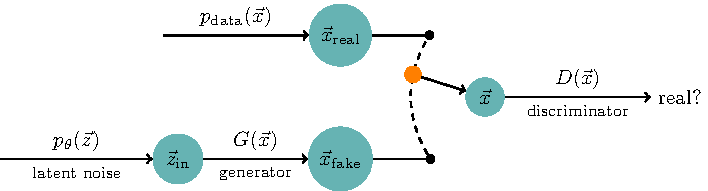
\includegraphics[width=\linewidth]{fig/generative_adversarial_nets.pdf}
    \caption{โมเดล Generative Adversarial Network (GAN) ซึ่งประกอบไปด้วย Generator และ Discriminator ซึ่งทั้งสอง%
    โมเดลเป็น Neural Network}
    \label{fig:gan}
\end{figure}

หลักการของ GAN คือโมเดลตัวแรกซึ่งเรียกว่า Generator จะสร้างข้อมูล (ปลอม) ที่มีลักษณะใกล้เคียงกันกับข้อมูลจริงขึ้นมา ในขณะที่โมเดล%
อีกตัวซึ่งเรีบกว่า Discriminator จะทำการแยกประเภทของข้อมูลที่เราต้องการโดยประเมินการทำงานของโมเดลตัวแรกโดยการตัดสินว่าข้อมูลที่ 
Generator สร้างขึ้นมานั้นมีความใกล้เคียงกับข้อมูลจริงมากน้อยแค่ไหน อธิบายให้ง่ายกว่านี้ก็คือโมเดลทั้งสองตัวนี้ถูกฝึกสอนให้ต่อสู้กันโดยที่
Generator นั้นพยายามสร้างข้อมูลหลอก Discriminator และ Discriminator ก็ต้องพยายามจับผิด Generator ให้ได้ โดยในภาพที่ 
\ref{fig:gan} แสดงองค์ประกอบของ GAN เริ่มต้นก็คือเรากำหนด Latent Noise ขึ้นมาก่อน แล้วให้ Generator นั้นสร้างข้อมูลปลอม 
($\vec{x}_{\text{fake}}$) โดยเรียนรู้จากข้อมูลจริง ($\vec{x}_{\text{real}}$) แล้ว Discriminator จะทำตรวจสอบต่อไป

ในปี ค.ศ. 2018 ได้มีการพัฒนา DeepFake ซึ่งเป็นปัญญาประดิษฐ์ที่สามารถสร้างภาพเคลื่อนไหวของบุคคลที่เราต้องการ โดยสามารถเลียน%
แบบทั้งท่าทาง, น้ำเสียง, ลักษณะการพูด, การขยับปาก แล้วนำข้อความที่เป็นเท็จใส่ลงไปให้เหมือนกับว่าเป็นคำพูดของบุคคลคนนั้น ทั้ง ๆ 
ที่บุคคลนั้นไม่ได้พูดประโยคเหล่านี้ออกมา สำหรับงานวิจัยทางด้านเคมีนั้นก็ได้มีการนำ GAN มาใช้ด้วยเช่นกัน เช่น การค้นหาโมเลกุลชนิดใหม่%
\autocite{prykhodko2019,lee2021,blanchard2021}, การทำนายโครงสร้างผลึกที่สภาวะต่าง ๆ\autocite{kim2020}, การออกแบบ%
สารประกอบอนินทรีย์\autocite{dan2020}, และการปรับปรุงการทำนายสเปกตรัม\autocite{al-mualem2022}

สำหรับงานวิจัยที่ใช้ GAN ที่ผู้เขียนจะยกมาให้ผู้อ่านได้ศึกษานั้นคือ \enquote{Generative Adversarial Networks for Transition State 
Geometry Prediction}\autocite{makos2021}

%--------------------------
\section{Transformer}
\label{sec:transformer}
\idxth{ตัวแปลง}
\idxen{Transformer}
%--------------------------

\begin{figure}[htbp]
    \centering
    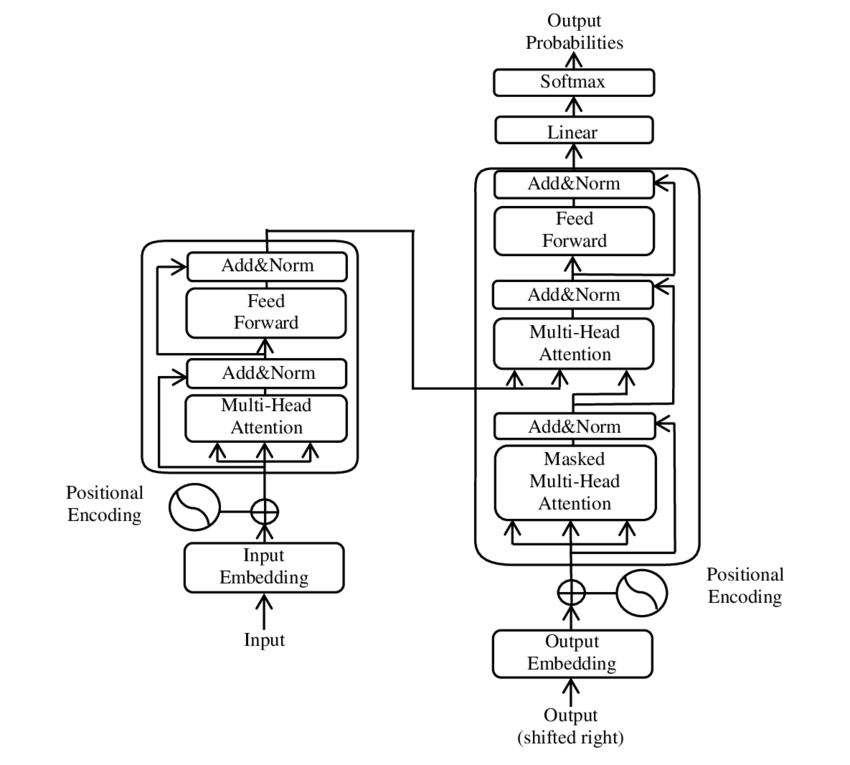
\includegraphics[width=\linewidth]{fig/transformer.png}
    \caption{สถาปัตยกรรมของโมเดล Transformer 
    (เครดิตภาพ: \url{https://en.wikipedia.org/wiki/Transformer_(machine_learning_model)})}
    \label{fig:transformer}
\end{figure}

ทรานส์ฟอร์มเมอร์ (Transformer)\autocite{vaswani2017a} เป็นโมเดล Neural Network ที่ถูกพัฒนาขึ้นมาเพื่อใช้ในการเรียนรู้ข้อมูลที่เป็น%
ลำดับ (Sequential Input) เช่น ข้อความหรือประโยค ซึ่งเหมือนกับโมเดล Recurrent Neural Network (RNN) ซึ่งมีประโยชน์อย่างมาก%
โดยเฉพาะการประยุกต์เพื่อการแปลภาษาจากภาษาหนึ่งไปยังอีกภาษาหนึ่ง รวมไปถึงการสรุปใจความสำคัญของประโยคหรือย่อหน้ายาว ๆ อย่างไรก็ตาม 
ปัญหาอย่างหนึ่งที่เป็นปัญหาสำคัญของการใช้ RNN ก็คือเรียนรู้ข้อมูลที่มีความต่อเนื่องกันยาว ๆ อย่างเช่นข้อความที่มีความซับซ้อนได้ไม่ดีนัก นั่นก็เพราะ%
ว่าสาเหตุก็คือข้อมูลที่ถูกส่งต่อจากอินพุตลำดับหนึ่งไปยังลำดับต่อ ๆ ไปนั้นสูญหายไประหว่างทาง จึงทำให้ประสิทธิภาพของการเรียนรู้ในการส่งต่อข้อมูลนั้น%
ทำได้ไม่ดีนัก

ด้วยเหตุนี้จึงเป็นที่มาของโมเดล Transformer ที่ถูกเสนอในปี ค.ศ. 2017 โดยทีมนักวิจัยจาก Google Brain ซึ่งได้ตีพิมพ์บทความงานวิจัยเรื่อง 
\enquote{Attention Is All You Need}\autocite{vaswani2017a} ซึ่งไอเดียของ Transformer ก็คือการใช้ Fully-Connected 
Neural Network แบบทั่วไปแล้วก็ใช้เพียงกลไกการใส่ใจ (Attention Mechanism) ซึ่งเป็นหัวใจหลักของโมเดลอันนี้ลยก็ว่าได้ โดย Attention 
Mechanism ได้เข้ามาช่วยทำให้ประสิทธิภาพของโมเดลนั้นดีกว่าโมเดล Sequence to Sequence (Seq2Seq) ที่ใช้ RNN นอกจากนี้ Transformer 
ยังมีข้อดีคือฝึกสอนโมเดลได้เร็วกว่า ใช้ทรัพยากรน้อยกว่า (ทำงานกับ GPU ได้ดีกว่า RNN ด้วย) และตีความการทำงานภายในได้ง่ายขึ้น รวมไปถึงการ%
แก้ปัญหา Vanishing Gradient ที่มักจะพบเจอใน RNN 

ภาพที่ \ref{fig:transformer} แสดงส่วนประกอบของโมเดล Transformer โดยมี Encoder ที่รับอินพุตที่เป็นลำดับข้อมูลเข้ามาและมี Decoder 
ที่รับเอาต์พุตที่เป็นลำดับ โดยในขั้นตอนการฝึกสอนโมเดลนี้ ลำดับข้อมูลของเอาต์พุตจะถูกเลื่อนไปทางขวาหนึ่งตำแหน่งซึ่งเป็นการฝึกสอนแบบ Teacher 
Forcing นั่นเอง

%--------------------------
\subsection{Attention}
\label{ssec:attention}
\idxen{Transformer!Attention}
%--------------------------

ตามที่ได้อธิบายไปก่อนหน้านี้ว่าเราสามารถออกแบบโมเดล Neural Machine Translation ให้มีความสามารถในการเรียนรู้ข้อมูลที่มีลำดับยาว ๆ 
ได้ด้วย Attention Mechanism โดยโมเดลจะโฟกัสเฉพาะบางส่วนของอินพุตเท่านั้น ณ เวลาหนึ่ง ซึ่งพารามิเตอร์ที่จะกำหนดการโฟกัสของโมเดลว่า%
จะโฟกัสที่ส่วนไหนนั้นก็จะได้จากการฝึกสอนโมเดลนั่นเอง

ประเภทของ Attention ที่ถูกนำมาใช้นั้นมีด้วยกัน 3 ประเภท ดังนี้

\begin{figure}[htbp]
    \centering
    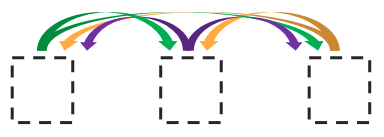
\includegraphics[width=0.6\linewidth]{fig/attention_1_self.png}
    \caption{Self-Attention (เครดิตภาพ: Łukasz Kaiser)}
    \label{fig:self_attention}
\end{figure}

\begin{figure}[htbp]
    \centering
    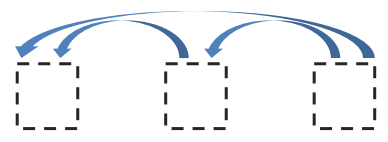
\includegraphics[width=0.6\linewidth]{fig/attention_2_masked.png}
    \caption{Masked Self-Attention (เครดิตภาพ: Łukasz Kaiser)}
    \label{fig:masked_self_attention}
\end{figure}

\begin{figure}[htbp]
    \centering
    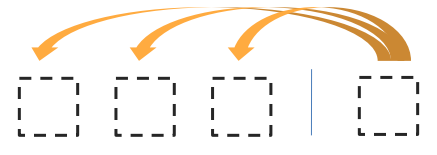
\includegraphics[width=0.6\linewidth]{fig/attention_3_enc-dec.png}
    \caption{Encoder-Decoder Attention (เครดิตภาพ: Łukasz Kaiser)}
    \label{fig:enc_dec_attention}
\end{figure}

\begin{enumerate}
    \item แบบแรกคือ Self-Attention โดยทุกหน่วยจะทำ Attention กับทุกหน่วย

    \item แบบที่สองคือ Masked Self-Attention โดยที่แต่ละหน่วยจะทำ Attention กับเฉพาะข้อมูลที่อยู่ลำดับก่อนหน้าเท่านั้น 
    โดย Attention ชนิดนี้จะใช้กับ Decoder เนื่องจากกระบวนการสร้างเอาต์พุตในตอนใช้งานจริงเป็นการสร้างทีละตัวจึงไม่สามารถนำข้อมูล%
    จากอนาคตมาใช้ได้

    \item แบบที่สามคือ Encoder-Decoder Attention เป็น Attention ที่เหมือนกับที่ใช้ในโมเดล seq2seq แบบทั่วไป โดยฝั่ง Decoder 
    จะเป็นตัวเรียกหรือดึงข้อมูล (Query) ข้อมูลมาจากฝั่ง Encoder
\end{enumerate}

%--------------------------
\subsection{Molecule Attention Transformer}
\label{ssec:mol_transformer}
\idxth{ตัวแปลง!ตัวแปลงความใส่ใจของโมเลกุล}
\idxen{Transformer!Molecule Attention Transformer}
%--------------------------

ตัวแปลงความใส่ใจของโมเลกุล (Molecule Attention Transformer หรือ MAT)\autocite{maziarka2020} เป็นโมเดลที่ใช้ Transformer
ในการพัฒนา

%--------------------------
\section{โมเดลอื่น ๆ}
\label{sec:other_ml_qm_models}
%--------------------------

นอกจากโมเดล ML ที่ได้อธิบายไปก่อนนี้ ยังมีอีกหลายโมเดลที่ถูกพัฒนาขึ้นมาเพื่อวัตถุประสงค์ที่แตกต่างกันไป โดยเฉพาะการทำนายคุณสมบัติของ%
โมเลกุลแบบเฉพาะเจาะจง โมเดล ML ที่ผู้อ่านสามารถศึกษาเพิ่มเติมเองได้มีดังนี้

\begin{table}[H]
    \centering
    \caption{โมเดล ML สำหรับเคมีควอนตัม}
    \label{tab:ml_qm_model}
    \begin{tabular}{cll}
    \toprule
    ปี ค.ศ. ที่ตีพิมพ์ &โมเดล ML &รายละเอียด \\
    \midrule
    2018 &DeePMD-kit\autocite{wang2018} &สำหรับคำนวณ Representation \\
    2019 &Cormorant\autocite{anderson2019} &สำหรับ Many-body System \\
    2020 &GMsNN\autocite{zaverkin2020} &ใช้ Gaussian Moment \\
    2021 &FieldSchNet\autocite{gastegger2021} &ปรับปรุง SchNet สำหรับการจำลองตัวทำละลาย \\
    2022 &DimeNet\autocite{gasteiger2022} &ใช้ Message-passing \\
    \bottomrule
    \end{tabular}
\end{table}
